\documentclass[3p]{elsarticle}
\usepackage{graphicx,pst-all}
\usepackage{epstopdf}
\usepackage{multirow}
\usepackage{xspace}
\usepackage{tabularx}
\usepackage{rotating}
\usepackage{float}
\usepackage{amsmath,amssymb,pifont}
\usepackage[mathscr]{eucal}
\usepackage[english,french]{babel}
\usepackage[T1]{fontenc}
\usepackage[utf8]{inputenc}
\usepackage{hyperref}

\newcommand{\n}{\tabularnewline}
\newcolumntype{C}{>{\centering}X}
\newcolumntype{R}{>{\raggedleft}X} 
\newcolumntype{L}{>{\raggedright}X} 
\newcolumntype{M}[1]{>{\centering}m{#1}}

\newenvironment{legend}%
 {\tabular{r>{\small} l}}%
 {\endtabular}

\newcommand{\Rm}[1]{{\bf R}_{#1}^{g+}}
\newcommand{\Rr}[1]{{\bf r}_{#1}^{g\ast}}
\newcommand{\Sm}[1]{{S_{#1}^{g+}}}
\newcommand{\Sr}[1]{{s_{#1}^{g\ast}}}
\newcommand{\Nr}[1]{N_{#1}^{\ast}}
\newcommand{\M}{\mathbb}
\newcommand{\B}[1]{{\bf #1}\xspace}
\newcommand{\T}{\texttt}
\newcommand{\Mc}{\mathcal}
\newcommand{\Hi}{\textit}
\newcommand{\norm}[1]{\left\|#1\right\|}
\newcommand{\abs}[1]{\left|#1\right|}
\newcommand{\snorm}[1]{\|#1\|}
\newcommand{\psca}[2]{\left\langle #1 , #2 \right\rangle}
\newcommand{\pscac}[2]{\textcolor{red}{\left\langle \textcolor{black}{#1} , \textcolor{black}{#2} \right\rangle}}
\newcommand{\la}{\Big\langle}
\newcommand{\ra}{\Big\rangle}
\newcommand{\im}{{\bf i}\xspace}
\newcommand{\sg}{\textrm{sg}}

\newcommand{\Eq}[1]{Eq.~\ref{eq:#1}}
\newcommand{\Eqs}[2]{Eqs.~\ref{eq:#1} et~\ref{eq:#2}}
\newcommand{\Eqss}[3]{Eqs.~\ref{eq:#1},~\ref{eq:#2} and~\ref{eq:#3}}
\newcommand{\Fig}[1]{Figure~\ref{fig:#1}}
\newcommand{\Figs}[2]{Figures~\ref{fig:#1} et~\ref{fig:#2}}
\newcommand{\Figss}[3]{Figures~\ref{fig:#1},~\ref{fig:#2} et~\ref{fig:#3}}
\newcommand{\Tab}[1]{Tableau~\ref{tab:#1}}
\newcommand{\Tabs}[2]{Tableaux~\ref{tab:#1} et~\ref{tab:#2}}
\newcommand{\Tabss}[3]{Tableaux~\ref{tab:#1},~\ref{tab:#2} et~\ref{tab:#3}}
\newcommand{\Sect}[1]{\S~\ref{sect:#1}}
\newcommand{\Sects}[2]{\S~\ref{sect:#1}~et~\ref{sect:#2}}
\newcommand{\Sec}[1]{\Sect{#1}}
\newcommand{\App}[1]{Annexe~\ref{app:#1}}
%\renewcommand{\emph}[1]{\textcolor{red}{\bf #1}}

\newenvironment{remark}[1][\textit{Nota Bene}]{\begin{trivlist}
\item[\hskip \labelsep {\bfseries \rule{1ex}{1ex} #1}]\ignorespaces}{\rule{1ex}{1ex} \end{trivlist}\ignorespacesafterend}

\newcounter{question}
\newcommand{\Q}[1]{\stepcounter{question}\begin{remark}[Q\arabic{question}]#1~~\end{remark}}

% notations
\newcommand{\functional}[2][\cdot]{\mathbb{#2}\left[#1\right]}
\newcommand{\function}[2][\cdot]{#2\left(#1\right)}
\newcommand{\grad}[1]{\nabla #1}
\newcommand{\dX}[1]{\frac{\partial #1}{\partial x}}
\renewcommand{\div}[1]{\nabla \cdot #1}
\newcommand{\Lapl}[1]{\Delta #1}
\newcommand{\LaplX}[1]{\frac{\partial^2 #1}{\partial x^2}}
\newcommand{\domain}[1]{V_{#1}}
\newcommand{\boundary}[1]{\partial \domain{#1}}
\newcommand{\interface}[1]{\Gamma_{#1}}
\DeclareMathOperator*{\argmin}{arg\,min}

\addto\captionsenglish{%
  \renewcommand{\abstractname}{Description}
}
\addto\captionsfrench{%
  \renewcommand{\abstractname}{Description}
}

\newenvironment{abstracts}
 {\global\setbox\absbox=\vbox\bgroup
    \hsize=\textwidth
    \linespread{1}\selectfont}
 {\vspace{-\bigskipamount}\egroup}
\renewenvironment{abstract}[1][]
 {\if\relax\detokenize{#1}\relax\else\selectlanguage{#1}\fi
  \noindent\textbf{\abstractname}\par\medskip\noindent\ignorespaces}
 {\par\bigskip}

 
\raggedbottom

\makeatletter
\def\ps@pprintTitle{
      \let\@oddhead\@empty
      \let\@evenhead\@empty
      \def\@oddfoot{\reset@font\hfil\thepage\hfil}
      \let\@evenfoot\@oddfoot
}
\makeatother
\bibliographystyle{elsarticle-num}

\begin{document}

\begin{frontmatter}

\title{TD: évaluation du bilan thermique intégral d'un bain de corium à deux couches}

% \author[LMAG]{R.~Le Tellier\corref{contact}}
% \ead{romain.le-tellier@cea.fr}
% \cortext[contact]{contact:}
% 
% \address[LMAG]{CEA, DEN, DTN/SMTA/LMAG, Cadarache \\
%   F-13108 Saint Paul-lez-Durance, France}
  
\begin{abstracts}
\selectlanguage{french}
\begin{abstract}[french]
%   Resum\'e en fran\c{c}ais
Dans ce TD, on se propose d'évaluer, à partir des hypothèses et fermetures classiquement utilisées dans les codes de calculs, la répartition de la puissance et du flux de chaleur aux interfaces d'un bain de corium dans une configuration stationnaire à deux couches: une phase oxyde qui porte toute la puissance résiduelle en-dessous d'une phase métallique. La phase oxyde est entourée d'une croûte réfractaire tandis que la phase métallique est en contact direct avec la paroi de la cuve en fusion. Il s'agit d'une adaptation de la configuration évaluée pour le réacteur AP1000 \cite{Esmaili2004} et reprise dans la série de benchmarks de \cite{Carenini2019}.
Pour faciliter la réalisation de ce TD (en particulier, les questions des \Sects{rad}{param} qui ne peuvent pas être traitées analytiquement), il est accompagné de notebooks Jupyter manipulable en ligne : \href[pdfnewwindow=true]{https://mybinder.org/v2/gh/niamorelreillet/ENSE3-Cours/main?urlpath=lab}{\color{blue}{\underline{\T{https://mybinder.org/v2/gh/niamorelreillet/ENSE3-Cours/main?urlpath=lab}}}}.
\end{abstract}
% \selectlanguage{english}
% \begin{abstract}
% %   Abstract in English 
% \end{abstract}
\end{abstracts}
  
\end{frontmatter}

\selectlanguage{french}

\section*{Préambule sur Jupyterlab}

Les notebooks Jupyter sont des cahiers électroniques qui, dans le même document, peuvent rassembler du texte, des images, des formules mathématiques et du code informatique exécutable (en l'occurence du python 3). Ils sont manipulables interactivement dans un navigateur web (voir, par exemple, \href{https://python.sdv.univ-paris-diderot.fr/18\_jupyter}{\color{blue}{\underline{\T{https://python.sdv.univ-paris-diderot.fr/18\_jupyter}}}}). 

Deux notebooks accompagnent ce TD :
\begin{itemize}
 \item \T{Very\_short\_python\_tutorial.ipynb}, un très court tutoriel qui montre les quelques fonctionnalités python nécessaires à la réalisation de ce TD ;
 \item \T{TD\_template.ipynb}, le ``canevas'' du TD à remplir en suivant les questions de l'énoncé ci-dessous ;
\end{itemize}

Ces notebooks peuvent être manipulés en ligne à l'adresse suivante : \\ \href[pdfnewwindow=true]{https://mybinder.org/v2/gh/niamorelreillet/ENSE3-Cours/main?urlpath=lab}{\color{blue}{\underline{\T{https://mybinder.org/v2/gh/niamorelreillet/ENSE3-Cours/main?urlpath=lab}}}}. 

La session ouverte par ce biais n'a qu'une durée de vie limitée mais, heureusement, il est possible de sauver 
\includegraphics[height=12pt]{Figures/binder_save.png} et restaurer 
\includegraphics[height=12pt]{Figures/binder_restore.png} les modifications faites au travers du stockage du navigateur web. Voir \href{https://discourse.jupyter.org/t/getting-your-notebook-after-your-binder-has-stopped/3268}{\color{blue}{\underline{\T{https://discourse.jupyter.org/t/getting-your-notebook-after-your-binder-has-stopped/3268}}}}. Il est conseillé d'utiliser Firefox ou Chrome comme navigateur web pour garantir la fonctionnement de cette fonctionnalité.

\begin{remark}
Bien sûr, si vous installez Jupyterlab sur votre ordinateur (par le biais d'Anaconda par exemple ; voir \href{https://test-jupyter.readthedocs.io/en/latest/install.html}{\color{blue}{\underline{\T{https://test-jupyter.readthedocs.io/en/latest/install.html}}}}), vous pouvez travailler localement
\end{remark}

Un troisième notebook (\T{TD.ipynb}), le TD complété, vous sera ``distribué'' à la fin.

\section*{Configuration, hypothèses, notations} \label{sect:sci}

La \Fig{2layer} présente la configuration considérée avec les notations associées vis-à-vis des flux de chaleur et des températures d'interface. Le fond de la cuve est hémisphérique de rayon $R=2$m. 

Les hypothèses simplificatrices suivantes seront faites vis-à-vis des couches liquides:
\begin{itemize}
 \item leur composition est uniforme;
 \item les fluides sont traités de manière incompressible sous l'hypothèse de Boussinesq;
 \item leur propriétés thermophysiques (hormis la masse volumique dans la flottabilité) ne dépendent pas de la température et sont données au \Tab{prop}.
\end{itemize}

Les hypothèses simplificatrices suivantes seront faites vis-à-vis de la croûte réfractaire entourant le bain oxyde:
\begin{itemize}
 \item sa composition est uniforme (et correspond à celle du solide formé à l'équilibre thermodynamique à la température de liquidus du liquide);
 \item sa masse sera négligée vis-à-vis de celle du liquide;
 \item la puissance volumique associée est considérée nulle;
 \item la conduction est considérée comme unidimensionnelle ``plan''.
\end{itemize}
On considèrera aussi que la conduction dans la paroi de la cuve est unidimensionnelle ``plan''.

Ecrivez-le bilan thermique des deux couches liquides en stationnaire. 

\Q{A partir des hypothèses précédentes, que pouvez-vous dire de $\phi_{up}^{ox}$ et $\phi_{met}^{dwn}$? Que cela implique-t-il pour la résolution du bilan thermique de ce bain à deux couches?}

\begin{figure}[H]
  \centering 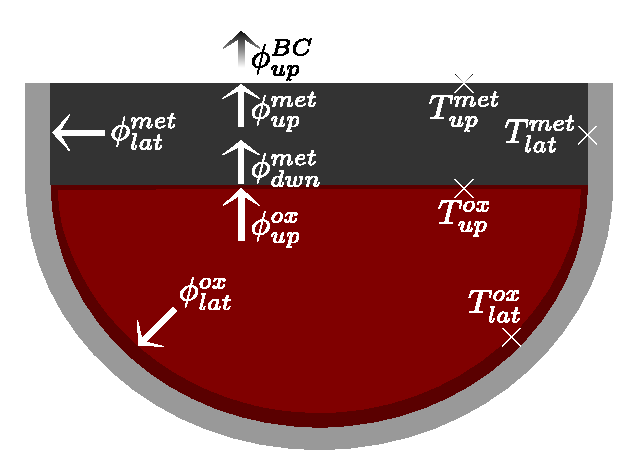
\includegraphics[height=0.4\textheight]{../Figures/TD_2layer.eps}
  \caption{Configuration à deux couches et notations des flux et températures} \label{fig:2layer}
\end{figure}

\begin{table}[H]
  \caption{Propriétés des deux phases liquides} \label{tab:prop}
  \centering \begin{tabularx}{0.9\textwidth}{|l|R|R|R|} \hline
  \multicolumn{1}{|c|}{\multirow{2}{*}{Propriété}} & \multicolumn{1}{c|}{\multirow{2}{*}{Unité}} & \multicolumn{2}{c|}{Valeur} \n
  & & \multicolumn{1}{c|}{Oxyde} & \multicolumn{1}{c|}{Métal} \n \hline
  masse volumique & kg.m$^{-3}$ & 8191 & 6899 \n
  conductivité thermique & W.m$^{-1}$.K$^{-1}$ & 5.3 & 25 \n
  viscosité cinématique & m$^2$s.$^{-1}$ & 5.7$\times$10$^{-7}$ & 5.9$\times$10$^{-7}$ \n
  capacité calorifique massique & J.K$^{-1}$.kg$^{-1}$ & 533 & 789.5 \n
  coefficient de dilatation thermique isobare & K$^{-1}$ & 1.05$\times$10$^{-4}$ & 1.11$\times$10$^{-4}$ \n
  température de liquidus & K & 2950 & 1600 \n
  puissance dissipée dans le volume & MW & 14 & 0 \n \hline
  \end{tabularx}
\end{table}

\begin{remark}
Dans tout ce qui suit, de par les corrélation utilisées, la longueur caractéristique qui intervient dans tous les nombres adimensionnels ($Ra_i$, $Ra$, $Nu$) est la hauteur de la couche concernée.
\end{remark}


\section{Bain oxyde}

Le bain oxyde occupe une hauteur $H^{ox}=1.5$m dans le fond de la cuve.

On cherche à calculer la température moyenne et la distribution de puissance entre surfaces latérale et supérieure à partir de l'équation d'énergie intégrale en stationnaire.

\Q{Calculer le volume \(V^{ox}\), la surface latérale \(S_{lat}^{ox}\) et la surface supérieure \(S_{up}^{ox}\)}
\Q{Calculer le nombre de Rayleigh interne \(Ra_i^{ox}\)}
\Q{Calculer le nombre de Nusselt associé à l'échange latéral \(Nu^{ox}_{lat}\) à partir de la corrélation ``BALI bas'' (\textit{cf.} \cite{Bonnet1999}) \(Nu^{ox}_{lat}=0.131\left(Ra_i^{ox}\right)^{0.25}\left(\frac{H^{ox}}{R}\right)^{0.19}\)}
\Q{Calculer le nombre de Nusselt associé à l'échange supérieur \(Nu^{ox}_{up}\) à partir de la corrélation ``BALI haut'' (\textit{cf.} \cite{Bonnet1999}) \(Nu^{ox}_{up}=0.381\left(Ra_i^{ox}\right)^{0.234}\)}
\Q{Calculer \(T^{ox}\)}
\Q{Calculer \(\phi_{lat}^{ox}\) et \(\phi_{up}^{ox}\) ainsi que la répartition de la puissance}

On considère maintenant que le flux latéral ``local'' \(\varphi_{lat}^{ox}(z)\) s'écrit \(\varphi_{lat}^{ox}(z) = \phi_{lat}^{ox} f(z)\) avec la fonction de forme $f(z)$ donnée par $\forall z \in [0,H^{ox}]$ :
\begin{equation}
 f(z)=0.25-0.75 \times c \times \cos^3(\theta)
\end{equation}
avec $\displaystyle \theta=\sin^{-1}\left(1-\frac{z}{R} \right)$, $\displaystyle \theta^{ox}=\sin^{-1}\left(1-\frac{H^{ox}}{R} \right)$ et $\displaystyle c = \frac{8\left(1-\sin\theta^{ox}\right)}{3\left(\frac{\pi}{2} - \theta^{ox}\right)-3\sin\theta^{ox}\cos\theta^{ox} - 2\sin\theta^{ox}\cos^3\theta^{ox}}$.

\Q{Tracer $\varphi_{lat}^{ox}(z)$ pour $z \in [0,H^{ox}]$ et comparer le maximum local de flux avec la valeur (pessimiste) de 1.5MW.m$^2$ du flux critique associé au refroidissement externe}


\section{Croûte réfractaire et ablation de la paroi cuve}

Pour une cote $z \in [0,H^{ox}]$ donnée, on considèrera que le flux ``local'' $\varphi_{lat}^{ox}(z)$ est dissipé par conduction unidimensionnelle ``plan'' dans l'épaisseur $e_c(z)$ de la croûte réfractaire et l'épaisseur $e_v(z)$ de la paroi de la cuve (\textit{cf.} \Fig{cv}). La paroi externe refroidie de la cuve sera supposée à une température constante $T_{lat}^{BC}=450$K.

On considèrera que la conductivité de la croûte $\lambda_c$ est la même que celle de la phase oxyde liquide tandis que, pour l'acier de la cuve, on prendra une conductivité $\lambda_v=40$W.m$^{-1}$.K$^{-1}$. Par ailleurs, la température de fusion de ce même acier sera prise égale à 1650K. Par ailleurs, l'épaisseur nominale de la paroi de la cuve est de 0.2$m$. 

\Q{En écrivant l'expression du flux conductif stationnaire dans l'épaisseur de la cuve, calculer la température $T_{c/v}$ d'interface entre la croûte et la cuve}

\Q{Quelle est la valeur maximale que peut atteindre $T_{c/v}$? En déduire l'épaisseur résiduelle $e_v(z)$ et la tracer selon $z$} (on ``ignorera'' l'acier fondu de la paroi de la cuve en considérant qu'il s'est relocalisé dans la couche métallique)

\Q{En écrivant l'expression du flux conductif stationnaire dans l'épaisseur de la croûte, calculer et tracer $e_c(z)$}


\begin{figure}[H]
\centering 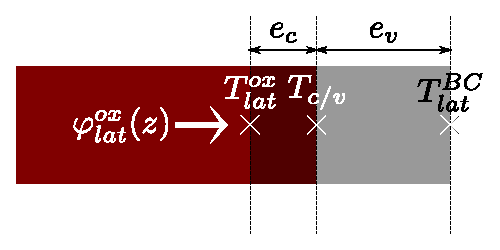
\includegraphics[width=0.5\textwidth]{Figures/crust_vessel.eps}
  \caption{Vue schématique de la conduction unidimensionnelle dans l'épaisseur de la croûte et la cuve pour une cote $z \in [0,H^{ox}]$ donnée} \label{fig:cv}
\end{figure}


\section{Couche métallique supérieure}

La couche métallique occupe une hauteur $H^{met}=0.9$m dans le fond de la cuve.

\Q{Calculer le nombre de Prandtl \(Pr^{met}\)}
\Q{Donner l'expression du nombre de Rayleigh externe \(Ra^{met}\left[\Delta T\right]\) et l'évaluer pour \(\Delta T=100\)K. Doit-on s'attendre à un écoulement laminaire ou turbulent?}
\Q{Calculer le volume \(V^{met}\), la surface latérale \(S_{lat}^{met}\) et la surface supérieure \(S_{up}^{met}\)}

On considèrera la corrélation de Globe\&Dropkin \cite{Globe1959} établie pour l'échange axial d’un liquide chauffé par le dessous et confinés entre deux plaques (resp. Chawla\&Chan \cite{Chawla1982} établie pour l'échange d’une paroi verticale immergée dans un fluide) pour le transfert en surface supérieure (resp. latérale):
\begin{quote}
\(Nu^{met}_{up}\left[\Delta T\right]=0.069\left(Pr^{met}\right)^{0.074}\left(Ra^{met}\left[\Delta T\right]\right)^{1/3}\)
\end{quote}
\begin{quote}
\(Nu^{met}_{lat}\left[\Delta T\right]=\frac{0.16}{\left(1+\left(\frac{0.492}{Pr^{met}}\right)^{9/16}\right)^{16/27}}\left(Ra^{met}\left[\Delta T\right]\right)^{1/3}\)
\end{quote}

\subsection{Condition adiabatique en surface supérieure}

Considérons d'abord une condition adiabatique en surface haute \textit{i.e.} \(\phi^{BC}_{up}=0\).

\Q{Calculer \(\phi_{lat}^{met}\)}
\Q{Calculer \(T^{met}\)}
 
\subsection{Condition de transfert radiatif en surface supérieure} \label{sect:rad}

Considérons maintenant un transfert radiatif en surface haute sous la forme simple suivante \(\phi^{BC}_{up}\left[T^{met}_{up}\right]=\varepsilon_{up}\sigma\left(\left(T^{met}_{up}\right)^4-\left(T^{BC}\right)^4\right)\)
où \(\varepsilon_{up}\) est une émissivité ``effective''.\footnote{e.g. pour un transfert entre deux plaques parallèles, \(\varepsilon_{up}=\left(\frac{1}{\varepsilon_1}+\frac{1}{\varepsilon_2}-1\right)^{-1}\)}

La résolution ne peut plus se faire de manière analytique.

\Q{Formaliser le problème à résoudre (deux équations, deux inconnues \(\left(T^{met},T_{up}^{met}\right)\)) et décrire l'algorithme que vous implémenteriez pour en trouver la solution}

\begin{remark} Pour la suite, l'accès aux notebooks Jupyter associé à ce TD est indispensable. Si ça n'est pas possible, une démonstration d'une telle résolution numérique sera faite et les résultats discutés. \end{remark}

\Q{En considérant $\varepsilon_{up} = 0.38$ et $T^{BC}=950$K, évaluer \(T^{met}\), \(T_{up}^{met}\), \(\phi_{lat}^{met}\) et \(\phi_{up}^{met}\)}

\subsection{Etudes paramétriques} \label{sect:param}

En considérant le cas avec transfert radiatif, on peut faire varier $\varepsilon_{up}$, $T^{BC}$ dans un premier temps, $H^{met}$ dans un second temps pour voir comment ça se comporte. Discuter de ces résultats vis-à-vis de la valeur (pessimiste) de 1.5MW.m$^2$ du flux critique associé au refroidissement externe.

\section*{Références}

\bibliography{../../References/lma-jabref.bib}

\end{document}